\documentclass{article}

\usepackage{graphicx}
\usepackage{tikz}
\usepackage{tikzsymbols}
\usetikzlibrary{calc,patterns,shapes.geometric}
\pagestyle{empty}
\usepackage[margin=0pt]{geometry}
\geometry{papersize={14in,12in}}

\def\centerarc[#1](#2)(#3:#4:#5){\draw[#1] ($(#2)+({#5*cos(#3)},{#5*sin(#3)})$) arc (#3:#4:#5);}

\begin{document}
	\begin{figure}
		\centering
		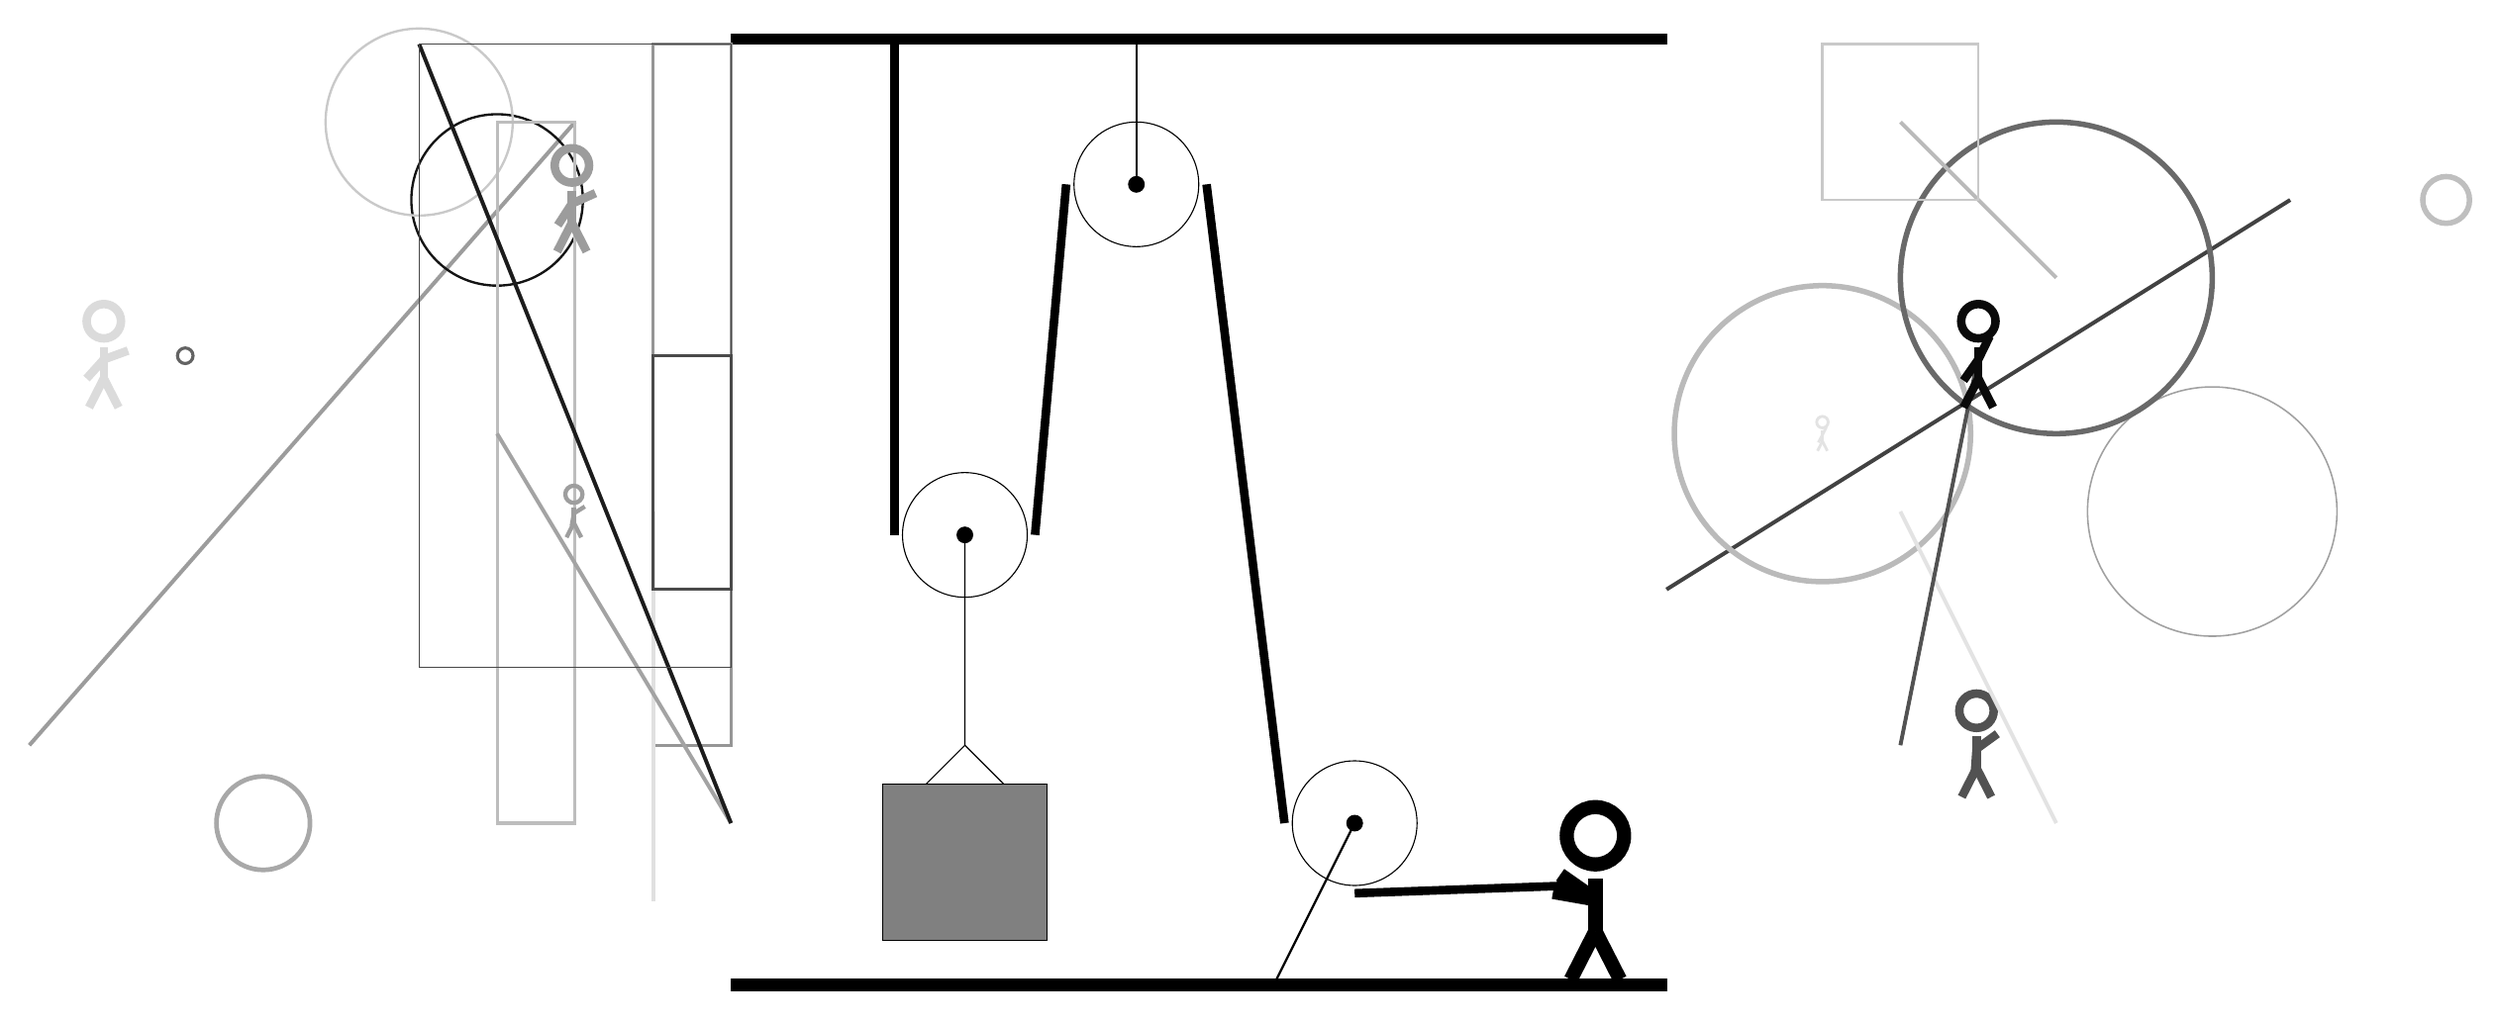
\begin{tikzpicture}
			%%%%% START %%%%%
			
			\draw[fill=black] (-2, 9) rectangle (10, 9.125);
			
			\draw[line width=0.5mm, color=black!39](-4, 8) -- (-11, 0);
			
			\draw[line width=0.5mm, color=black!74](10, 2) -- (18, 7);
			\draw [line width=0.2mm, color=black!37](17, 3) circle (1.6);
			\draw[line width=0.4mm, color=black!41] (-2, 0) rectangle (-3, 9);
			\draw [line width=0.3mm, color=black!92](-5, 7) circle (1.1);
			\draw [line width=0.7mm, color=black!25](20, 7) circle (0.3);
			\draw [line width=0.7mm, color=black!27](12, 4) circle (1.9);
			\node[line width=0.4mm, color=black!11] at (12, 4) {\Strichmaxerl[2][62][63]};
			\node[line width=0.3mm, color=black!68] at (14, 0) {\Strichmaxerl[6][86][36]};
			\draw[line width=0.5mm, color=black!12](-3, -2) -- (-3, 3);
			\draw [line width=0.3mm, color=black!21](-6, 8) circle (1.2);
			\draw[line width=0.4mm, color=black!26] (-4, -1) rectangle (-5, 8);
			\draw [line width=0.7mm, color=black!59](15, 6) circle (2.0);
			\draw [line width=0.2mm, color=black!67](11, 3) circle (0.0);
			\draw[line width=0.5mm, color=black!36](-5, 4) -- (-2, -1);
			\node[line width=0.3mm, color=black!38] at (-4, 3) {\Strichmaxerl[3][80][32]};
			
			\draw[line width=0.5mm, color=black!89](-6, 9) -- (-2, -1);
			\draw [line width=0.6mm, color=black!34](-8, -1) circle (0.6);
			\draw[line width=0.5mm, color=black!27](13, 8) -- (15, 6);
			\draw[line width=0.5mm, color=black!11](15, -1) -- (13, 3);
			\draw[line width=0.5mm, color=black!68](13, 0) -- (14, 5);
			
			\node[line width=0.2mm, color=black!14] at (-10, 5) {\Strichmaxerl[6][48][20]};
			\draw[line width=0.3mm, color=black!21] (12, 7) rectangle (14, 9);
			\draw[line width=0.2mm, color=black!72] (-2, 9) rectangle (-6, 1);
			\node[line width=0.5mm, color=black!96] at (14, 5) {\Strichmaxerl[6][55][64]};
			\draw[line width=0.6mm, color=black!74] (-4, 4) rectangle (-4, 4);
			
			\draw[line width=0.4mm, color=black!71] (-2, 2) rectangle (-3, 5);
			\draw [line width=0.4mm, color=black!61](-9, 5) circle (0.1);
			\node[line width=0.4mm, color=black!39] at (-4, 7) {\Strichmaxerl[6][57][24]};
			
			\draw (3.2, 7.2) circle (0.8);
			\draw[fill=black] (3.2, 7.2) circle (0.1);
			\draw[thick] (3.2, 7.2) -- (3.2, 9);
			
			\draw (6, -1) circle (0.8);
			\draw[fill=black] (6, -1) circle (0.1);
			\draw[thick] (6, -1) -- (5, -3);
			
			\draw (1, 2.7) circle (0.8);
			\draw[fill=black] (1, 2.7) circle (0.1);
			
			\draw (1, 2.7) -- (1, 0) -- (0.5, -0.5);
			\draw (1, 0) -- (1.5, -0.5);
			\draw[fill=black!50] (-0.05, -0.5) rectangle (2.05, -2.5);
			
			\draw[line width=1.1mm] (0.1, 9) -- (0.1, 2.7);
			\centerarc[line width=1.1mm](1, 2.7)(180:360:0.9);
			\draw[line width=1.1mm](1.9, 2.7) -- (2.3, 7.2);
			\centerarc[line width=1.1mm](3.2, 7.2)(0:180:0.9);
			\draw[line width=1.1mm](4.1, 7.2) -- (5.1, -1);
			\centerarc[line width=1.1mm](6, -1)(180:270:0.9);
			\draw[line width=1.1mm](6, -1.9) -- (8.8, -1.8);
			
			\node at (9, -1.9) {\Strichmaxerl[10][-35][170]};
			
			\draw[fill=black] (-2, -3) rectangle (10, -3.15);
			
			%%%%% END %%%%%
		\end{tikzpicture}
	\end{figure}	
\end{document}